% !TEX TS-program = pdflatex
% !TEX encoding = UTF-8 Unicode

% This is a simple template for a LaTeX document using the "article" class.
% See "book", "report", "letter" for other types of document.

\documentclass[8pt]{article} % use larger type; default would be 10pt

\usepackage[utf8]{inputenc} % set input encoding (not needed with XeLaTeX)
\usepackage{bchart}
\usepackage{longtable}
\usepackage{pgfgantt}
\usepackage{calendar} % Use the calendar.sty style
\usepackage{calc}
\usepackage{ifthen}
\usepackage{tkz-base}
\usepackage{tikz}
\usepackage{hyperref}
\usepackage{tkz-kiviat,numprint,fullpage} 
\usepackage{pgfplotstable} 
\usetikzlibrary{arrows}
\RequirePackage{pgfcalendar}
\RequirePackage{tikz}
\usetikzlibrary{%
arrows, backgrounds, calc,%
patterns, positioning, shapes.geometric%
}
%%% Examples of Article customizations
% These packages are optional, depending whether you want the features they provide.
% See the LaTeX Companion or other references for full information.

\usepackage{textcomp}
%\usepackage{hyperref}

%%% PAGE DIMENSIONS
\usepackage{geometry} % to change the page dimensions
\geometry{a4paper} % or letterpaper (US) or a5paper or....
% \geometry{margin=2in} % for example, change the margins to 2 inches all round
% \geometry{landscape} % set up the page for landscape
%   read geometry.pdf for detailed page layout information

\usepackage{graphicx} % support the \includegraphics command and options

% \usepackage[parfill]{parskip} % Activate to begin paragraphs with an empty line rather than an indent

%%% PACKAGES
\usepackage{booktabs} % for much better looking tables
\usepackage{array} % for better arrays (eg matrices) in maths
\usepackage{paralist} % very flexible & customisable lists (eg. enumerate/itemize, etc.)
\usepackage{verbatim} % adds environment for commenting out blocks of text & for better verbatim
\usepackage{subfig} % make it possible to include more than one captioned figure/table in a single float
% These packages are all incorporated in the memoir class to one degree or another...

%%% HEADERS & FOOTERS
\usepackage{fancyhdr} % This should be set AFTER setting up the page geometry
\pagestyle{fancy} % options: empty , plain , fancy
\renewcommand{\headrulewidth}{0pt} % customise the layout...
\lhead{}\chead{}\rhead{}
\lfoot{}\cfoot{\thepage}\rfoot{}

%%% SECTION TITLE APPEARANCE
\usepackage{sectsty}
\allsectionsfont{\sffamily\mdseries\upshape} % (See the fntguide.pdf for font help)
% (This matches ConTeXt defaults)

%%% ToC (table of contents) APPEARANCE
\usepackage[nottoc,notlof,notlot]{tocbibind} % Put the bibliography in the ToC
\usepackage[titles,subfigure]{tocloft} % Alter the style of the Table of Contents
\renewcommand{\cftsecfont}{\rmfamily\mdseries\upshape}
\renewcommand{\cftsecpagefont}{\rmfamily\mdseries\upshape} % No bold!

%%% END Article customizations

%%% The "real" document content comes below...

\title{Project management}
\author{\copyright Frederic Kerdraon}
%\date{} % Activate to display a given date or no date (if empty),
         % otherwise the current date is printed 

\begin{document}
\maketitle
\tableofcontents

\section{Introduction}

This document summurizes all the important informations necessary to facilitate things and remove a lot of stress. It's been put together thanks to \LaTeX. This is designed to help make optimal decisions for a not so short lifetime.

%{\footnote
%Ce n'est pas parceque les choses sont difficiles que nous n'osons pas, c'est parceque nous n'osons pas qu'elles sont difficiles
%}
%{\footnote
%For once you have tasted flight you will walk the earth with your eyes turned skywards, 
%for there you have been and there you will long to return.
%Leonardo da Vinci
%
%}
%\makebox[2\width]{hello}

\newcounter{a}
\newcounter{b}

%----------------------------------------------------------
\newcommand{\slice}[4]{
  \pgfmathparse{0.5*#1+0.5*#2}
  \let\midangle\pgfmathresult

   slice
  \draw[thick,fill=black!10] (0,0) -- (#1:1) arc (#1:#2:1) -- cycle;

   outer label
  \node[label=\midangle:#4] at (\midangle:1) {};

   inner label
  \pgfmathparse{min((#2-#1-10)/110*(-0.3),0)}
  \let\temp\pgfmathresult
  \pgfmathparse{max(\temp,-0.5) + 0.8}
  \let\innerpos\pgfmathresult
  \node at (\midangle:\innerpos) {#3};
}

\section{Management summary}

Historical cumulated income and charges

\begin{figure}[ht!]
\centering
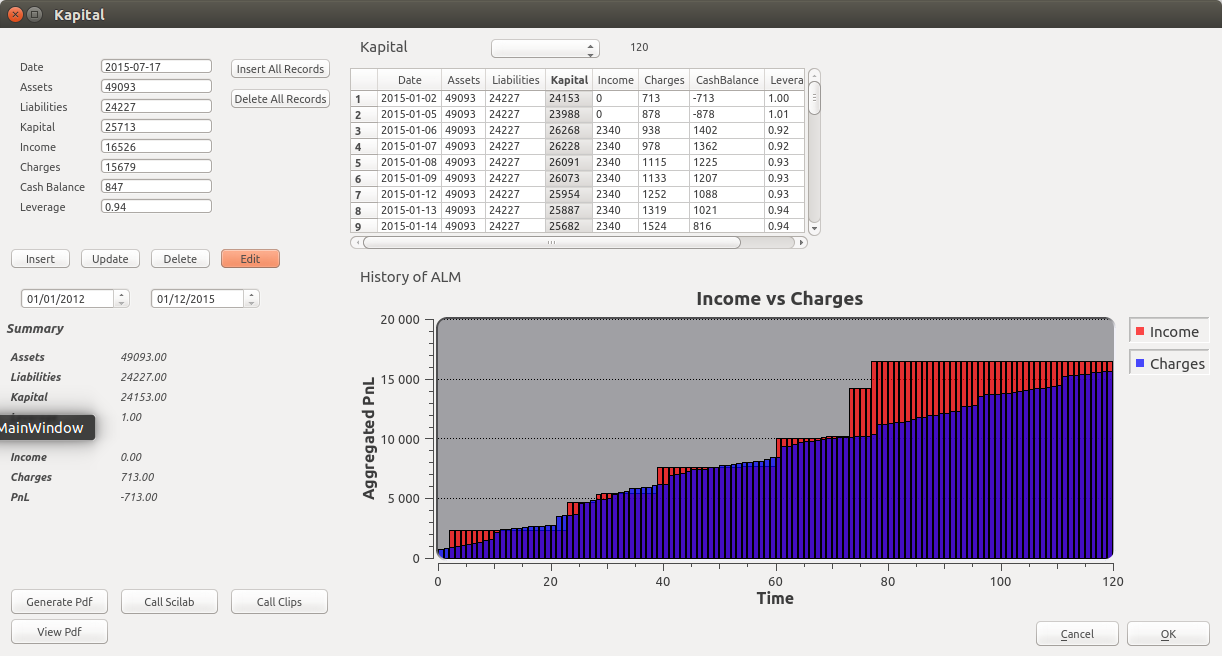
\includegraphics[width=120mm]{Kapital2.png}
\caption{A simple caption \label{overflow}}
\end{figure}

%{\footnote
%En gros tous les dossiers que j'ai au bureau....;-)
%}


\subsection{Summary}

\subsubsection{The green side first !}
Tasks that we couldnt complete in time\\
Highest investment or Budget (time and monney)\\
Resources that deserve hols\\
Tasks that we dont want to fuck up (critical path of the highest investment)\\

\subsubsection{The new challenges ahead !}
Highest investment or Budget (time and monney)\\
Tasks that we couldnt complete in time\\
Resources that need to move their asses\\
Tasks that we dont want to fuck up (critical path of the highest investment)\\

\subsection{Events}
From events (Meetings, Deliverables)
\begin{longtable}{|c|c|c|c|}
\hline
\multicolumn{4}{|c|}{Events} \\
\hline
Date & Type & Name & Template\\
\hline
Monday January 2013 & Deliverable & Inception & \\
\hline
Monday January 2013 & Deliverable & Specification & \\
\hline
Monday January 2013 & Deliverable & Clearchoice & \\
\hline
Monday January 2013 & Deliverable & External design & \\
\hline
Monday January 2013 & Deliverable & Internal design & \\
\hline
Monday January 2013 & Deliverable & Test documentation & \\
\hline
Monday January 2013 & Deliverable & Release notes & \\
\hline
Monday January 2013 & Deliverable & Post implementation review & \\
\hline
Monday January 2013 & Deliverable & Support documentation & \\
\hline
Monday January 2013 & Deliverable & Inception & \\
\hline
Monday January 2013 & Deliverable & Specification & \\
\hline
Monday January 2013 & Deliverable & Clearchoice & \\
\hline
Monday January 2013 & Deliverable & External design & \\
\hline
Monday January 2013 & Deliverable & Internal design & \\
\hline
Monday January 2013 & Deliverable & Test documentation & \\
\hline
Monday January 2013 & Deliverable & Release notes & \\
\hline
Monday January 2013 & Deliverable & Post implementation review & \\
\hline
Saturday November 2013 & Deliverable & Support documentation & \\
\hline
Friday November 2013 & Birthday & Annif Antoine & \\
\hline
Thursday October 2013 & Meeting & Council & Council.tex\\
\hline
Wednesday June 2014 & Meeting & Council & Council.tex\\
\hline
Monday December 2015 & Daily & Daily setup & ManagementSummary.pdf\\
\hline
Monday December 2015 & Daily & Daily setup & ManagementSummary.pdf\\
\hline
Monday December 2015 & Event & Renouvellement Assu Auto & Letter.pdf\\
\hline
Sunday December 2015 & Event & Renouvellement Assu Bateau & Letter.pdf\\
\hline
Sunday December 2015 & Event & Renouvellement Assu Maison & Letter.pdf\\
\hline
Saturday December 2015 & Event & Revision auto & Letter.pdf\\
\hline
Saturday December 2015 & Event & Renouvellement carte paiement & Letter.pdf\\
\hline
Friday December 2015 & Event & Declaration impots & Letter.pdf\\
\hline
Friday December 2015 & Event & Paiement des impots & Letter.pdf\\
\hline
Thursday December 2015 & Event & Arbre de noel & Letter.pdf\\
\hline
 ... & ... & ... & ... \\
\hline
\hline
\end{longtable}


\subsubsection{Tasks aggregated}
Ajouter time to expiry, Feasible time, Feasible Budget, Feasible Complexity/Risks
RAF, Done, Completion perc, Maturity\\
\begin{longtable}{|c|c|c|}
\hline
\multicolumn{3}{|c|}{Tasks} \\
\hline
Project & ROI & Complexity \\
\hline
Finance & 35082 & 12\\
\hline
Friends & 12601 & 30\\
\hline
Work & 500 & 4\\
\hline
Boat & 332 & 269\\
\hline
Day to day & 2 & 30\\
\hline
Done & 1 & 2\\
\hline
Car & 0 & 3\\
\hline
Plijadur & 0 & 3\\
\hline
Pending & 0 & 1\\
\hline
 & 0 & 1\\
\hline
\end{longtable}

\begin{bchart}[min=0,max=350,step=70,unit=k\texteuro]
\bcbar[label=Finance]{350}\\
\smallskip
\bcbar[label=Friends]{126}\\
\smallskip
\bcbar[label=Work]{5}\\
\smallskip
\bcbar[label=Boat]{3}\\
\smallskip
\bcbar[label=Day to day]{0}\\
\smallskip
\bcbar[label=Done]{0}\\
\smallskip
\bcbar[label=Car]{0}\\
\smallskip
\bcbar[label=Plijadur]{0}\\
\smallskip
\bcbar[label=Pending]{0}\\
\smallskip
\bcbar[label=]{0}\\
\smallskip
\end{bchart}


%\subsubsection{Tasks 3D burndown}
%\begin{tikzpicture}
\begin{axis}[3d box,xmin=-5,xmax=5,ymin=-5,ymax=5,width=9cm,height=9.25cm,grid=both, minor z tick num=1]
\addplot3 graphics[points={%
(-4.4449,4.6547,0) => (110.814,167.827)
(-4.633,-4.5186,0) => (264.187,74.679)
(4.5829,-4.5216,0) => (470.558,145.343)
(-0.45821,-0.43355,1157) => (287.474,379.016)
}]
{Project.png};
\node at (axis cs:-1.5,0.5,490) [inner sep=0pt, pin={[pin edge={thick,black},align=left]145:Interesting\\Data Point}] {};
\end{axis}
\end{tikzpicture}

\subsubsection{Tasks 3D burndown}
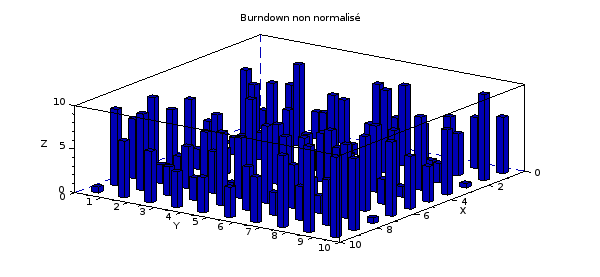
\includegraphics[width=1\textwidth]{Project.png}

\subsubsection{Tasks detailed}
{\footnotesize
\begin{longtable}{|c|c|c|c|c|c|}
\hline
\multicolumn{6}{|c|}{Tasks} \\
\hline
Project & Task & Return & Cost & R/C & NumDays \\
\hline
Boat & Sell Plijadur & 15000 & 1 & 15000 & 10\\
\hline
IT & Qt - add global update for tasks from Qt & 1000 & 1 & 1000 & 10\\
\hline
Climate camp & visiter les terrains et poser des jalons & 750 & 1 & 750 & 10\\
\hline
Friends & Diner Armelle & 3200 & 5 & 640 & 10\\
\hline
Friends & Diner Christophe & 1200 & 2 & 600 & 10\\
\hline
Work & Meet guys fromTyfab & 500 & 1 & 500 & 10\\
\hline
Work & Meet guys fromTyfab & 500 & 1 & 500 & 10\\
\hline
Friends & D�jeuner Karel & 4000 & 10 & 400 & 10\\
\hline
Friends & Diner Zaz & 3800 & 10 & 380 & 10\\
\hline
Friends & Diner Jab & 400 & 2 & 200 & 10\\
\hline
Boat & Sale genoa36 & 150 & 1 & 150 & 10\\
\hline
Boat & Motor servicing & 100 & 1 & 100 & 10\\
\hline
Boat & Careen the Boat & 90 & 1 & 90 & 10\\
\hline
Finance & HSBC transfer & 80 & 1 & 80 & 10\\
\hline
Boat & Genoa - crowd funding? & 50 & 1 & 50 & 10\\
\hline
Plijadur & Plastify maps & 40 & 1 & 40 & 10\\
\hline
Plijadur & Plastify maps & 40 & 1 & 40 & 10\\
\hline
Boat & Buy masks & 40 & 1 & 40 & 10\\
\hline
Boat & Write log book - for history & 35 & 1 & 35 & 10\\
\hline
Plijadur & Copy all the movies from toto/film & 20 & 1 & 20 & 10\\
\hline
Plijadur & Copy all the movies from toto/film & 20 & 1 & 20 & 10\\
\hline
Boat & Build workbench2 & 20 & 1 & 20 & 10\\
\hline
Plijadur & Copy all the movies from toto/Big bang & 10 & 1 & 10 & 10\\
\hline
Plijadur & Copy all the movies from toto/Big bang & 10 & 1 & 10 & 10\\
\hline
Guitar & Change the strings & 87 & 25 & 3.48 & 10\\
\hline
Boat & Install the GPS & 20 & 7 & 2.85714285714286 & 10\\
\hline
Plijadur & Prof de guitare & 30 & 20 & 1.5 & 10\\
\hline
Plijadur & Prof de guitare & 30 & 20 & 1.5 & 10\\
\hline
Boat & Chang lamps & 10 & 8 & 1.25 & 10\\
\hline
Boat & Clean the freezer & 10 & 9 & 1.11111111111111 & 10\\
\hline
Finance & Check weird bank transfers & 1 & 1 & 1 & 10\\
\hline
Boat & Remove radio from the boat & 1 & 1 & 1 & 10\\
\hline
Finance & Contact EDF & 1 & 1 & 1 & 10\\
\hline
Friends & Call Phil & 1 & 1 & 1 & 10\\
\hline
Day to day & Buy lighter gaz & 1 & 1 & 1 & 10\\
\hline
Guitar & Change the strings & 58 & 89 & 0.651685393258427 & 10\\
\hline
Boat & Install a line on the fishing rod & 1 & 14 & 0.0714285714285714 & 10\\
\hline
Boat & Clean the deck & 1 & 15 & 0.0666666666666667 & 10\\
\hline
Boat & Grease the helm & 1 & 16 & 0.0625 & 10\\
\hline
Boat & Clean the sofas & 1 & 17 & 0.0588235294117647 & 10\\
\hline
Boat & Clean the inox & 1 & 18 & 0.0555555555555556 & 10\\
\hline
Boat & Check the anchorage & 1 & 20 & 0.05 & 10\\
\hline
Boat & Install sound & 1 & 22 & 0.0454545454545455 & 10\\
\hline
Boat & Check battery connexions & 1 & 23 & 0.0434782608695652 & 10\\
\hline
Boat & Fix the 12v on the rack & 1 & 24 & 0.0416666666666667 & 10\\
\hline
Boat & Change camping stove support & 1 & 25 & 0.04 & 10\\
\hline
Boat & Varnish the woods & 1 & 28 & 0.0357142857142857 & 10\\
\hline
IT & Data - Check the numbers & 0 & 1 & 0 & 10\\
\hline
Admin & Check references & 0 & 1 & 0 & 10\\
\hline
Health & Contact Jean Mich & 0 & 1 & 0 & 10\\
\hline
Health & Contacter Laurent Le bras & 0 & 1 & 0 & 10\\
\hline
Health & Go horse riding & 0 & 1 & 0 & 10\\
\hline
IT & Qt - Add combo box category for tasks & 0 & 1 & 0 & 10\\
\hline
Health & Find a badminton spot & 0 & 1 & 0 & 10\\
\hline
IT & Copy researchwork to office desktop & 0 & 1 & 0 & 10\\
\hline
IT & Qt - plug the graphs (all of them) & 0 & 1 & 0 & 10\\
\hline
IT & Scanner & 0 & 1 & 0 & 10\\
\hline
IT & Multiplex sound & 0 & 1 & 0 & 10\\
\hline
IT & Mysql - Check data  & 0 & 1 & 0 & 10\\
\hline
IT & Mysql - Generate Ids automatically & 0 & 1 & 0 & 10\\
\hline
IT & Qt - add update for tasks & 0 & 1 & 0 & 10\\
\hline
IT & Qt - add delete row tasks & 0 & 1 & 0 & 10\\
\hline
IT & Implement Clips & 0 & 1 & 0 & 10\\
\hline
IT & Implement Android (On the laptop) & 0 & 1 & 0 & 10\\
\hline
IT & Perl - Get global variables & 0 & 1 & 0 & 10\\
\hline
IT & Find protection N95 & 0 & 1 & 0 & 10\\
\hline
IT & Scan photos & 0 & 1 & 0 & 10\\
\hline
IT & Qt - try to get progress bar to move & 0 & 1 & 0 & 10\\
\hline
IT & Qt - Add combo box status for tasks & 0 & 1 & 0 & 10\\
\hline
Project & Weight & 0 & 1 & 0 & 10\\
\hline
Project & Weight & 0 & 1 & 0 & 10\\
\hline
Project & Weight & 0 & 1 & 0 & 10\\
\hline
Project & Weight & 0 & 1 & 0 & 10\\
\hline
Project & Weight & 0 & 1 & 0 & 10\\
\hline
Project & Weight & 0 & 1 & 0 & 10\\
\hline
Project & Weight & 0 & 1 & 0 & 10\\
\hline
Project & Weight & 0 & 1 & 0 & 10\\
\hline
Project & Weight & 0 & 1 & 0 & 10\\
\hline
Project & Weight & 0 & 1 & 0 & 10\\
\hline
Project & Weight & 0 & 1 & 0 & 10\\
\hline
Project & Weight & 0 & 1 & 0 & 10\\
\hline
Project & Weight & 0 & 1 & 0 & 10\\
\hline
Project & Weight & 0 & 1 & 0 & 10\\
\hline
Project & Weight & 0 & 1 & 0 & 10\\
\hline
Project & Weight & 0 & 1 & 0 & 10\\
\hline
IT & Qt - Add small calendar for start and end dates & 0 & 1 & 0 & 10\\
\hline
Project & Weight & 0 & 1 & 0 & 10\\
\hline
Project & Weight & 0 & 1 & 0 & 10\\
\hline
IT & Qt - Add combo box prority for tasks & 0 & 1 & 0 & 10\\
\hline
IT & Qt - Add small calendar for start and end dates & 0 & 1 & 0 & 10\\
\hline
IT & Scilab - Manage interpolation & 0 & 1 & 0 & 10\\
\hline
IT & Qt - add completion for tasks research & 0 & 1 & 0 & 10\\
\hline
IT & Joomla - Fill in the pages automatically & 0 & 1 & 0 & 10\\
\hline
t &  & 0 & 1 & 0 & 10\\
\hline
IT & Joomla - Implement an insert into the database & 0 & 1 & 0 & 10\\
\hline
IT & Qt update colors of tasks depending on priority & 0 & 1 & 0 & 10\\
\hline
IT & Installer NetBeans & 0 & 1 & 0 & 10\\
\hline
IT & Add the nice graph to the Stocks paper & 0 & 1 & 0 & 10\\
\hline
t &  & 0 & 1 & 0 & 10\\
\hline
t &  & 0 & 1 & 0 & 10\\
\hline
t &  & 0 & 1 & 0 & 10\\
\hline
t &  & 0 & 1 & 0 & 10\\
\hline
t &  & 0 & 1 & 0 & 10\\
\hline
Project & Weight & 0 & 1 & 0 & 10\\
\hline
Project & Weight & 0 & 1 & 0 & 10\\
\hline
Project & Weight & 0 & 1 & 0 & 10\\
\hline
Guitar & Clean the Startocaster & 0 & 54 & 0 & 10\\
\hline
Climate camp & Plant seeds & 0 & 1 & 0 & 10\\
\hline
Guitar & Clean the Startocaster & 0 & 54 & 0 & 10\\
\hline
Admin & List accesses & 0 & 1 & 0 & 10\\
\hline
Climate camp & Plant seeds & 0 & 1 & 0 & 10\\
\hline
Finance & Pay Alfa & 0 & 1 & 0 & 10\\
\hline
Admin & Manage historical revenues & 0 & 1 & 0 & 10\\
\hline
Admin & Transfert MDP agenda 2014 & 0 & 1 & 0 & 10\\
\hline
Admin & Declare revenues & 0 & 1 & 0 & 10\\
\hline
Day to day & Use lifting barr & 0 & 1 & 0 & 10\\
\hline
Boat & Build workbench & 0 & 1 & 0 & 10\\
\hline
Day to day & Buy a camping chair & 0 & 1 & 0 & 10\\
\hline
Day to day & Add birthdays on the calendar & 0 & 1 & 0 & 10\\
\hline
Admin & Sell guitar stand & 0 & 1 & 0 & 10\\
\hline
Admin & Regroup contacts by town & 0 & 1 & 0 & 10\\
\hline
Day to day & Check for storage & 0 & 1 & 0 & 10\\
\hline
Day to day & Polish glasses & 0 & 1 & 0 & 10\\
\hline
IT & Add Linux & News & Sports & Admin & 0 & 1 & 0 & 10\\
\hline
Admin & Add St Meen to the calendrier & 0 & 1 & 0 & 10\\
\hline
Admin & Pay baillif for the Castel harbour & 0 & 1 & 0 & 10\\
\hline
Climate camp & visiter les terrains et poser des jalons & 0 & 1 & 0 & 10\\
\hline
Boat & Make winter covers for Plijadur & 0 & 1 & 0 & 10\\
\hline
Guitar & Change the strings & 0 & 1 & 0 & 10\\
\hline
Guitar & Prices index & 0 & 53 & 0 & 10\\
\hline
Boat & Complete description & 0 & 1 & 0 & 10\\
\hline
Boat & Link to the vendor - http://www.jeanneau.fr/ & 0 & 1 & 0 & 10\\
\hline
Boat & Percentage Broker & 0 & 1 & 0 & 10\\
\hline
Boat & Clean up external company & 0 & 1 & 0 & 10\\
\hline
Boat & Price 30 & 0 & 1 & 0 & 10\\
\hline
Boat & For sale Jeanneau & 0 & 1 & 0 & 10\\
\hline
Boat & Photo Facebook + Photos Blog + Videos & 0 & 1 & 0 & 10\\
\hline
IT & Check the size of the pictures and homogenize & 0 & 1 & 0 & 10\\
\hline
Guitar & Prices index & 0 & 53 & 0 & 10\\
\hline
Boat & Interior clean up & 0 & 1 & 0 & 10\\
\hline
Finance & Update LinkedIn & 0 & 1 & 0 & 10\\
\hline
Day to day & Get back stuff Jessica & 0 & 1 & 0 & 10\\
\hline
Day to day & scanners les docs & 0 & 1 & 0 & 10\\
\hline
Day to day & Photos of my stuff & 0 & 1 & 0 & 10\\
\hline
Day to day & Add consumption to the IT tools & 0 & 1 & 0 & 10\\
\hline
Day to day & Make list of books & 0 & 1 & 0 & 10\\
\hline
Boat & Write log book & 0 & 1 & 0 & 10\\
\hline
Day to day & Find back crew Plijadur & 0 & 1 & 0 & 10\\
\hline
Day to day & Ben Harper tatoo & 0 & 1 & 0 & 10\\
\hline
Health & Create a football team & 0 & 1 & 0 & 10\\
\hline
Day to day & Contact PHD & 0 & 1 & 0 & 10\\
\hline
Day to day & Call Christine & 0 & 1 & 0 & 10\\
\hline
Finance & Sell guitar & 0 & 1 & 0 & 10\\
\hline
Finance & Calculate Australian project & 0 & 1 & 0 & 10\\
\hline
Finance & Meeting taxes & 0 & 1 & 0 & 10\\
\hline
Finance & Get a lawyer & 0 & 1 & 0 & 10\\
\hline
Day to day & Get the musculation stuff up stairs & 0 & 1 & 0 & 10\\
\hline
Day to day & Buy guitar Titi & 0 & 1 & 0 & 10\\
\hline
Boat & Sale genoa & 0 & 1 & 0 & 10\\
\hline
Boat & Check keel & 0 & 1 & 0 & 10\\
\hline
Boat & Rent of the boat & 0 & 1 & 0 & 10\\
\hline
Boat & Check VHF & 0 & 1 & 0 & 10\\
\hline
Boat & Check nautical maps & 0 & 1 & 0 & 10\\
\hline
Boat & Sale genoa Lorient & 0 & 1 & 0 & 10\\
\hline
Boat & Repair electric rack & 0 & 1 & 0 & 10\\
\hline
Car & Faire reparer la clim de l'alfa & 0 & 1 & 0 & 10\\
\hline
Car & Clean up the car & 0 & 1 & 0 & 10\\
\hline
Day to day & Buy black gloves & 0 & 1 & 0 & 10\\
\hline
Day to day & Installer musculation engine & 0 & 1 & 0 & 10\\
\hline
Day to day & Get back the portable freeezer & 0 & 1 & 0 & 10\\
\hline
Day to day & Get back tools from Zaz & 0 & 1 & 0 & 10\\
\hline
Day to day & Acheter cadre & 0 & 1 & 0 & 10\\
\hline
Car & Change oil & 0 & 1 & 0 & 10\\
\hline

\begin{bchart}[min=0,max=50,step=10,unit=k\texteuro]
\bcbar[label=Sell Plijadur]{15}\\
\smallskip
\bcbar[label=Qt - add global update for tasks from Qt]{1}\\
\smallskip
\bcbar[label=visiter les terrains et poser des jalons]{0}\\
\smallskip
\bcbar[label=Diner Armelle]{3}\\
\smallskip
\bcbar[label=Diner Christophe]{1}\\
\smallskip
\bcbar[label=Meet guys fromTyfab]{0}\\
\smallskip
\bcbar[label=Meet guys fromTyfab]{0}\\
\smallskip
\bcbar[label=D�jeuner Karel]{4}\\
\smallskip
\bcbar[label=Diner Zaz]{3}\\
\smallskip
\bcbar[label=Diner Jab]{0}\\
\smallskip
\bcbar[label=Sale genoa36]{0}\\
\smallskip
\bcbar[label=Motor servicing]{0}\\
\smallskip
\bcbar[label=Careen the Boat]{0}\\
\smallskip
\bcbar[label=HSBC transfer]{0}\\
\smallskip
\bcbar[label=Genoa - crowd funding?]{0}\\
\smallskip
\bcbar[label=Plastify maps]{0}\\
\smallskip
\bcbar[label=Plastify maps]{0}\\
\smallskip
\bcbar[label=Buy masks]{0}\\
\smallskip
\bcbar[label=Write log book - for history]{0}\\
\smallskip
\bcbar[label=Copy all the movies from toto/film]{0}\\
\smallskip
\bcbar[label=Copy all the movies from toto/film]{0}\\
\smallskip
\bcbar[label=Build workbench2]{0}\\
\smallskip
\bcbar[label=Copy all the movies from toto/Big bang]{0}\\
\smallskip
\bcbar[label=Copy all the movies from toto/Big bang]{0}\\
\smallskip
\bcbar[label=Change the strings]{0}\\
\smallskip
\bcbar[label=Install the GPS]{0}\\
\smallskip
\bcbar[label=Prof de guitare]{0}\\
\smallskip
\bcbar[label=Prof de guitare]{0}\\
\smallskip
\bcbar[label=Chang lamps]{0}\\
\smallskip
\bcbar[label=Clean the freezer]{0}\\
\smallskip
\bcbar[label=Check weird bank transfers]{0}\\
\smallskip
\bcbar[label=Remove radio from the boat]{0}\\
\smallskip
\bcbar[label=Contact EDF]{0}\\
\smallskip
\bcbar[label=Call Phil]{0}\\
\smallskip
\bcbar[label=Buy lighter gaz]{0}\\
\smallskip
\bcbar[label=Change the strings]{0}\\
\smallskip
\bcbar[label=Install a line on the fishing rod]{0}\\
\smallskip
\bcbar[label=Clean the deck]{0}\\
\smallskip
\bcbar[label=Grease the helm]{0}\\
\smallskip
\bcbar[label=Clean the sofas]{0}\\
\smallskip
\bcbar[label=Clean the inox]{0}\\
\smallskip
\bcbar[label=Check the anchorage]{0}\\
\smallskip
\bcbar[label=Install sound]{0}\\
\smallskip
\bcbar[label=Check battery connexions]{0}\\
\smallskip
\bcbar[label=Fix the 12v on the rack]{0}\\
\smallskip
\bcbar[label=Change camping stove support]{0}\\
\smallskip
\bcbar[label=Varnish the woods]{0}\\
\smallskip
\bcbar[label=Data - Check the numbers]{0}\\
\smallskip
\bcbar[label=Check references]{0}\\
\smallskip
\bcbar[label=Contact Jean Mich]{0}\\
\smallskip
\bcbar[label=Contacter Laurent Le bras]{0}\\
\smallskip
\bcbar[label=Go horse riding]{0}\\
\smallskip
\bcbar[label=Qt - Add combo box category for tasks]{0}\\
\smallskip
\bcbar[label=Find a badminton spot]{0}\\
\smallskip
\bcbar[label=Copy researchwork to office desktop]{0}\\
\smallskip
\bcbar[label=Qt - plug the graphs (all of them)]{0}\\
\smallskip
\bcbar[label=Scanner]{0}\\
\smallskip
\bcbar[label=Multiplex sound]{0}\\
\smallskip
\bcbar[label=Mysql - Check data ]{0}\\
\smallskip
\bcbar[label=Mysql - Generate Ids automatically]{0}\\
\smallskip
\bcbar[label=Qt - add update for tasks]{0}\\
\smallskip
\bcbar[label=Qt - add delete row tasks]{0}\\
\smallskip
\bcbar[label=Implement Clips]{0}\\
\smallskip
\bcbar[label=Implement Android (On the laptop)]{0}\\
\smallskip
\bcbar[label=Perl - Get global variables]{0}\\
\smallskip
\bcbar[label=Find protection N95]{0}\\
\smallskip
\bcbar[label=Scan photos]{0}\\
\smallskip
\bcbar[label=Qt - try to get progress bar to move]{0}\\
\smallskip
\bcbar[label=Qt - Add combo box status for tasks]{0}\\
\smallskip
\bcbar[label=Weight]{0}\\
\smallskip
\bcbar[label=Weight]{0}\\
\smallskip
\bcbar[label=Weight]{0}\\
\smallskip
\bcbar[label=Weight]{0}\\
\smallskip
\bcbar[label=Weight]{0}\\
\smallskip
\bcbar[label=Weight]{0}\\
\smallskip
\bcbar[label=Weight]{0}\\
\smallskip
\bcbar[label=Weight]{0}\\
\smallskip
\bcbar[label=Weight]{0}\\
\smallskip
\bcbar[label=Weight]{0}\\
\smallskip
\bcbar[label=Weight]{0}\\
\smallskip
\bcbar[label=Weight]{0}\\
\smallskip
\bcbar[label=Weight]{0}\\
\smallskip
\bcbar[label=Weight]{0}\\
\smallskip
\bcbar[label=Weight]{0}\\
\smallskip
\bcbar[label=Weight]{0}\\
\smallskip
\bcbar[label=Qt - Add small calendar for start and end dates]{0}\\
\smallskip
\bcbar[label=Weight]{0}\\
\smallskip
\bcbar[label=Weight]{0}\\
\smallskip
\bcbar[label=Qt - Add combo box prority for tasks]{0}\\
\smallskip
\bcbar[label=Qt - Add small calendar for start and end dates]{0}\\
\smallskip
\bcbar[label=Scilab - Manage interpolation]{0}\\
\smallskip
\bcbar[label=Qt - add completion for tasks research]{0}\\
\smallskip
\bcbar[label=Joomla - Fill in the pages automatically]{0}\\
\smallskip
\bcbar[label=]{0}\\
\smallskip
\bcbar[label=Joomla - Implement an insert into the database]{0}\\
\smallskip
\bcbar[label=Qt update colors of tasks depending on priority]{0}\\
\smallskip
\bcbar[label=Installer NetBeans]{0}\\
\smallskip
\bcbar[label=Add the nice graph to the Stocks paper]{0}\\
\smallskip
\bcbar[label=]{0}\\
\smallskip
\bcbar[label=]{0}\\
\smallskip
\bcbar[label=]{0}\\
\smallskip
\bcbar[label=]{0}\\
\smallskip
\bcbar[label=]{0}\\
\smallskip
\bcbar[label=Weight]{0}\\
\smallskip
\bcbar[label=Weight]{0}\\
\smallskip
\bcbar[label=Weight]{0}\\
\smallskip
\bcbar[label=Clean the Startocaster]{0}\\
\smallskip
\bcbar[label=Plant seeds]{0}\\
\smallskip
\bcbar[label=Clean the Startocaster]{0}\\
\smallskip
\bcbar[label=List accesses]{0}\\
\smallskip
\bcbar[label=Plant seeds]{0}\\
\smallskip
\bcbar[label=Pay Alfa]{0}\\
\smallskip
\bcbar[label=Manage historical revenues]{0}\\
\smallskip
\bcbar[label=Transfert MDP agenda 2014]{0}\\
\smallskip
\bcbar[label=Declare revenues]{0}\\
\smallskip
\bcbar[label=Use lifting barr]{0}\\
\smallskip
\bcbar[label=Build workbench]{0}\\
\smallskip
\bcbar[label=Buy a camping chair]{0}\\
\smallskip
\bcbar[label=Add birthdays on the calendar]{0}\\
\smallskip
\bcbar[label=Sell guitar stand]{0}\\
\smallskip
\bcbar[label=Regroup contacts by town]{0}\\
\smallskip
\bcbar[label=Check for storage]{0}\\
\smallskip
\bcbar[label=Polish glasses]{0}\\
\smallskip
\bcbar[label=Add Linux & News & Sports & Admin]{0}\\
\smallskip
\bcbar[label=Add St Meen to the calendrier]{0}\\
\smallskip
\bcbar[label=Pay baillif for the Castel harbour]{0}\\
\smallskip
\bcbar[label=visiter les terrains et poser des jalons]{0}\\
\smallskip
\bcbar[label=Make winter covers for Plijadur]{0}\\
\smallskip
\bcbar[label=Change the strings]{0}\\
\smallskip
\bcbar[label=Prices index]{0}\\
\smallskip
\bcbar[label=Complete description]{0}\\
\smallskip
\bcbar[label=Link to the vendor - http://www.jeanneau.fr/]{0}\\
\smallskip
\bcbar[label=Percentage Broker]{0}\\
\smallskip
\bcbar[label=Clean up external company]{0}\\
\smallskip
\bcbar[label=Price 30]{0}\\
\smallskip
\bcbar[label=For sale Jeanneau]{0}\\
\smallskip
\bcbar[label=Photo Facebook + Photos Blog + Videos]{0}\\
\smallskip
\bcbar[label=Check the size of the pictures and homogenize]{0}\\
\smallskip
\bcbar[label=Prices index]{0}\\
\smallskip
\bcbar[label=Interior clean up]{0}\\
\smallskip
\bcbar[label=Update LinkedIn]{0}\\
\smallskip
\bcbar[label=Get back stuff Jessica]{0}\\
\smallskip
\bcbar[label=scanners les docs]{0}\\
\smallskip
\bcbar[label=Photos of my stuff]{0}\\
\smallskip
\bcbar[label=Add consumption to the IT tools]{0}\\
\smallskip
\bcbar[label=Make list of books]{0}\\
\smallskip
\bcbar[label=Write log book]{0}\\
\smallskip
\bcbar[label=Find back crew Plijadur]{0}\\
\smallskip
\bcbar[label=Ben Harper tatoo]{0}\\
\smallskip
\bcbar[label=Create a football team]{0}\\
\smallskip
\bcbar[label=Contact PHD]{0}\\
\smallskip
\bcbar[label=Call Christine]{0}\\
\smallskip
\bcbar[label=Sell guitar]{0}\\
\smallskip
\bcbar[label=Calculate Australian project]{0}\\
\smallskip
\bcbar[label=Meeting taxes]{0}\\
\smallskip
\bcbar[label=Get a lawyer]{0}\\
\smallskip
\bcbar[label=Get the musculation stuff up stairs]{0}\\
\smallskip
\bcbar[label=Buy guitar Titi]{0}\\
\smallskip
\bcbar[label=Sale genoa]{0}\\
\smallskip
\bcbar[label=Check keel]{0}\\
\smallskip
\bcbar[label=Rent of the boat]{0}\\
\smallskip
\bcbar[label=Check VHF]{0}\\
\smallskip
\bcbar[label=Check nautical maps]{0}\\
\smallskip
\bcbar[label=Sale genoa Lorient]{0}\\
\smallskip
\bcbar[label=Repair electric rack]{0}\\
\smallskip
\bcbar[label=Faire reparer la clim de l'alfa]{0}\\
\smallskip
\bcbar[label=Clean up the car]{0}\\
\smallskip
\bcbar[label=Buy black gloves]{0}\\
\smallskip
\bcbar[label=Installer musculation engine]{0}\\
\smallskip
\bcbar[label=Get back the portable freeezer]{0}\\
\smallskip
\bcbar[label=Get back tools from Zaz]{0}\\
\smallskip
\bcbar[label=Acheter cadre]{0}\\
\smallskip
\bcbar[label=Change oil]{0}\\
\smallskip

}

%\subsubsection{ROI}
\subsubsection{Sponsors}
%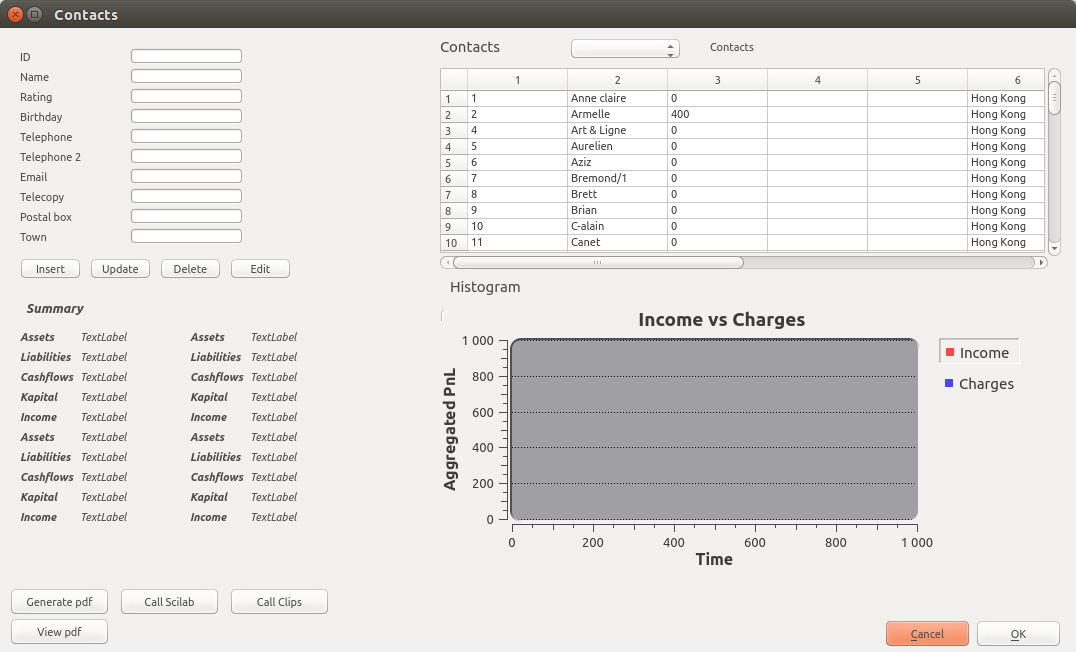
\includegraphics[width=90mm]{Contacts.png}
%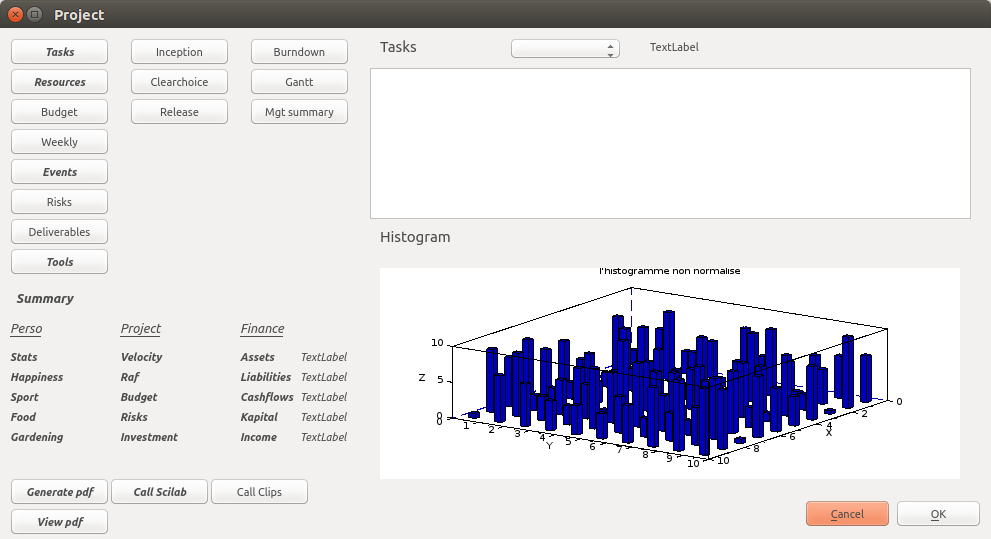
\includegraphics[width=90mm]{Projects.png}
%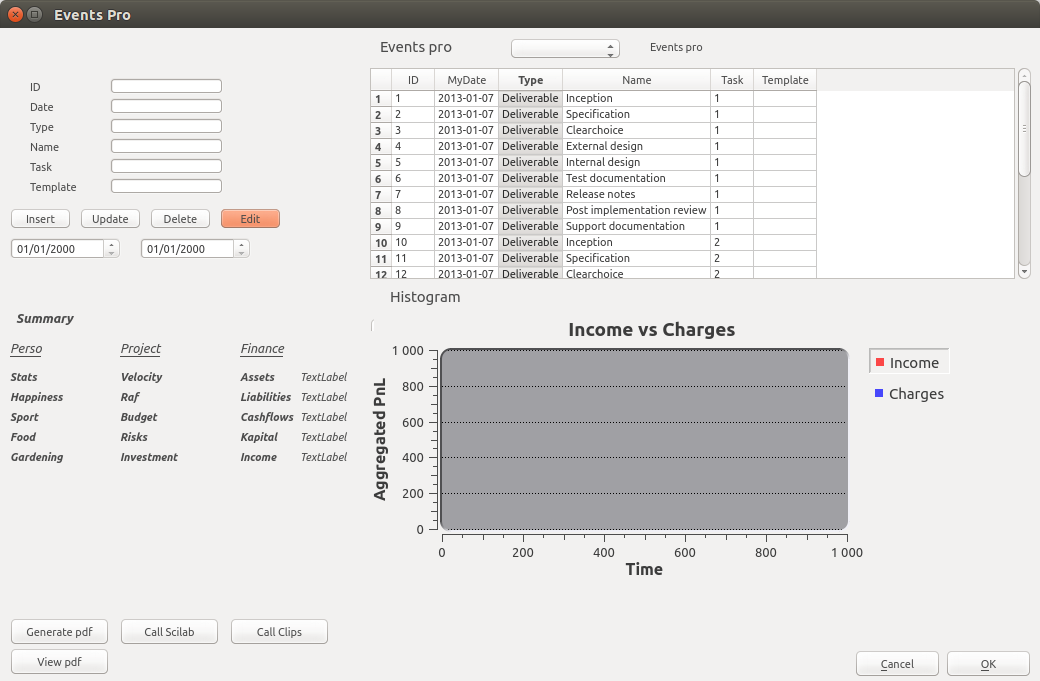
\includegraphics[width=90mm]{EventsPro.png}
%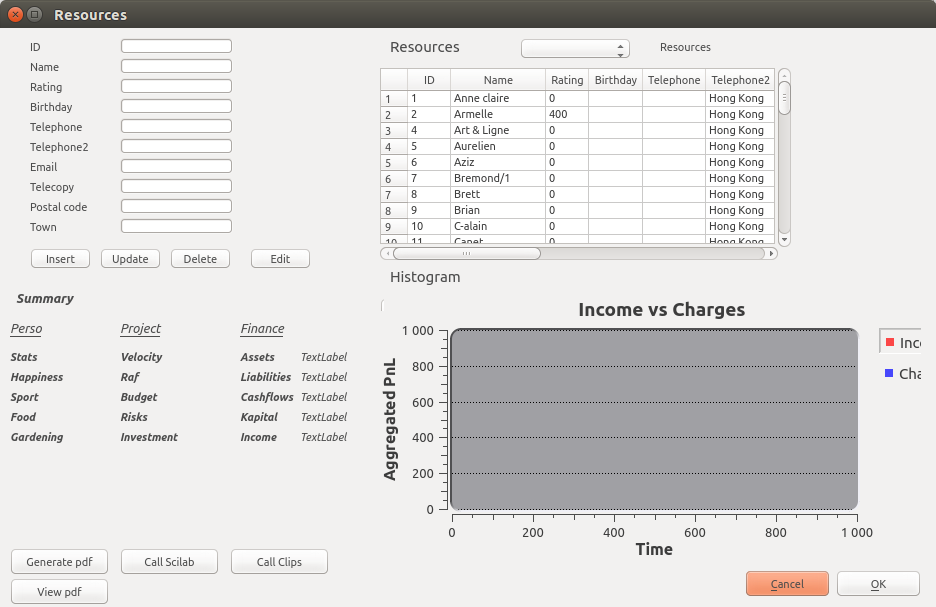
\includegraphics[width=90mm]{Resources.png}
%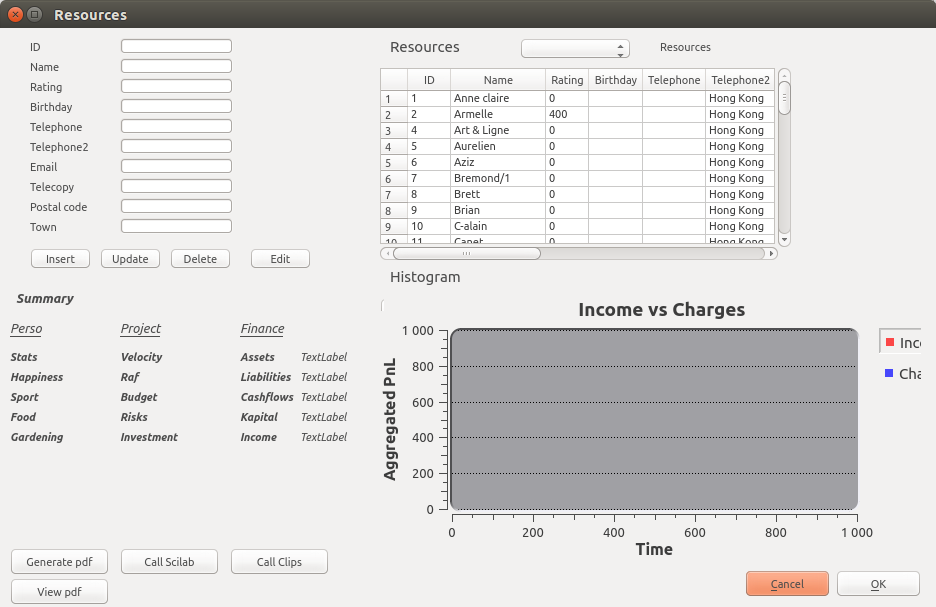
\includegraphics[width=90mm]{Resources.png}
\begin{tikzpicture}
\tkzKiviatDiagramFromFile[
        scale=.5,
        label distance=.5cm,
        gap     = 1,
        label space=3,  
        lattice = 10]{assets.dat}
\tkzKiviatLineFromFile[thick,
                       color      = blue,
                       mark       = ball,
                       ball color = blue,
                       mark size  = 4pt,
                       fill       = blue!20]{assets.dat}{2}
\tkzKiviatLineFromFile[thick,
                       color      = red,
                       mark       = ball,
                       ball color = red,
                       mark size  = 4pt,
                       fill       = red!20]{assets.dat}{1}     
\end{tikzpicture}

%\subsubsection{Budget}
%From Tasks.csv
\subsubsection{Risks}
Not enough budget, Not enough resources (including me)
\subsubsection{Targets}
From Gantt
\subsubsection{Propositions from Artificial Intelligence}
From Gantt
%\subsubsection{Table}


\section{Associated Project Management}

From now on we focus on one single project, else it's gonna be messie 
\subsection{Deliverables}
From events.csv
\subsection{Gantt}
Pour que le Gantt soit a sa place!!!!!
\begin{tikzpicture}
\begin
{
ganttchart
}[
y unit title=0.4cm,
y unit chart=0.5cm,
vgrid,
time slot format=isodate-yearmonth,
compress calendar,
title/.append style={draw=none, fill=RoyalBlue!50!black},
title label font=
\sffamily
\bfseries
\color
{white},
title label node/.append style={below=-1.6ex},
title left shift=.05,
title right shift=-.05,
title height=1,
bar/.append style={draw=none, fill=OliveGreen!75},
bar height=.6,
bar label font=
\normalsize
\color
{black!50},
group right shift=0,
group top shift=.6,
group height=.3,
group peaks height=.2,
bar incomplete/.append style={fill=Maroon}
]{2010-09}{2011-12}
\gantttitlecalendar
{year} \\
\ganttbar
[
progress=100,
bar progress label font=
\small
\color
{OliveGreen!75},
bar progress label node/.append style={right=4pt},
bar label font=
\normalsize
\color
{OliveGreen},
name=pp
]{Preliminary Project}{2010-09}{2010-12} \\
\ganttset
{progress label text={}, link/.style={black, -to}}
\ganttgroup
{Objective 1}{2011-01}{2011-12} \\
\ganttbar
[progress=4, name=T1A]{Task A}{2011-01}{2011-06} \\
\ganttlinkedbar
[progress=0]{Task B}{2011-07}{2011-12} \\
\ganttgroup
{Objective 2}{2011-01}{2011-12} \\
\ganttbar
[progress=15, name=T2A]{Task A}{2011-01}{2011-09} \\
\ganttlinkedbar
[progress=0]{Task B}{2011-10}{2011-12} \\
\ganttgroup
{Objective 3}{2011-05}{2011-08} \\
\ganttbar
[progress=0]{Task A}{2011-05}{2011-08}
\ganttset
{link/.style={OliveGreen}}
\ganttlink
[link mid=.4]{pp}{T1A}
\ganttlink
[link mid=.159]{pp}{T2A}
\end
{
ganttchart
}
\end{tikzpicture}

%#####################################################################################

\subsection{Burn down}
From tasks.csv + Dispo weekly of each resource
%Graphique\\
\\
Calcul de vitesse\\
s=speed\\
p=position\\
n=number of units\\
t=time\\
s=n/t\\
\\
Projection lineaire\\
y=s*x+p\\
Theoretical end\\


%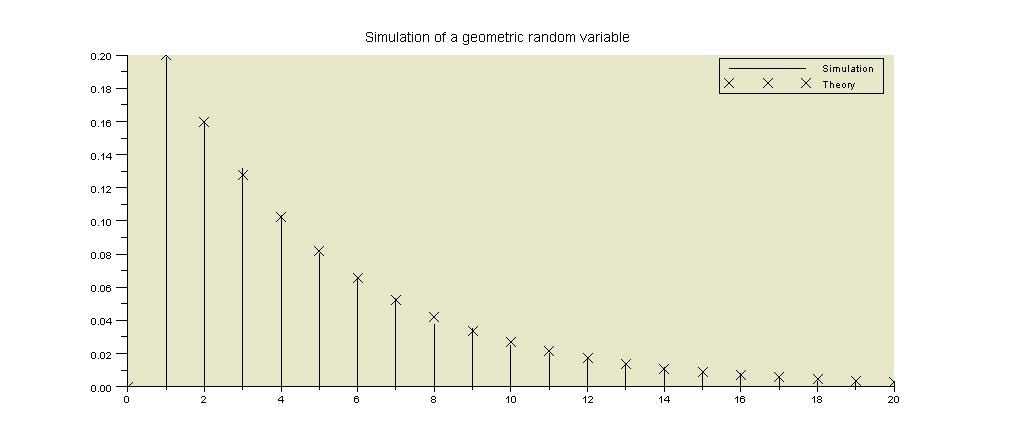
\includegraphics[width=20pts]{Geometric.jpg}



\subsection{Resources}

Top 10 resources to take care of\\
Workload (days, percentage time, stress, fatigue sum of days without break, ambition)
Diagramme en etoile per deliverable\\
Rates for all the resources

\subsubsection{Data}
\begin{longtable}{|c|c|c|c|c|}
\hline
\multicolumn{5}{|c|}{Contacts} \\
\hline
ID & Name & Rating & Town & Telephone\\
\hline
101 & Wing & 1000 & HongKong & 85296001395\\
\hline
108 & Zazzy & 900 & Brest & 33611037735\\
\hline
27 & Flozio & 850 & Brest & 33680938975\\
\hline
24 & Fanch & 800 & Brest & 33685769214\\
\hline
68 & Mummy & 800 & Brest & 33674340108\\
\hline
89 & Sonia & 600 & Rennes & 33612425946\\
\hline
83 & Rico & 550 & Brest & 33611037992\\
\hline
60 & Maeva & 500 & Brest & 33662575512\\
\hline
42 & Jessie & 500 & Brest & 33681775660\\
\hline
41 & Jessica & 500 & Brest & 699114929\\
\hline
23 & Etienne & 400 & Brest & 619144832\\
\hline
2 & Armelle & 400 & Brest & 33677134026\\
\hline
96 & Tiprig & 250 & Paris & 33663626188\\
\hline
22 & Elise & 250 & ???? & 33614921085\\
\hline
 ... & ... & ... & ... & ... \\
\hline
Total & 8300 &  & & \\
\hline
\end{longtable}

%\subsubsection{Graph}
%\begin{bchart}[min=0,max=1000,step=200,unit=K\texteuro]
\bcbar[label=Wing]{1000}\\
\smallskip
\bcbar[label=Zazzy]{900}\\
\smallskip
\bcbar[label=Flozio]{850}\\
\smallskip
\bcbar[label=Fanch]{800}\\
\smallskip
\bcbar[label=Mummy]{800}\\
\smallskip
\bcbar[label=Sonia]{600}\\
\smallskip
\bcbar[label=Rico]{550}\\
\smallskip
\bcbar[label=Maeva]{500}\\
\smallskip
\bcbar[label=Jessie]{500}\\
\smallskip
\bcbar[label=Jessica]{500}\\
\smallskip
\bcbar[label=Etienne]{400}\\
\smallskip
\bcbar[label=Armelle]{400}\\
\smallskip
\bcbar[label=Tiprig]{250}\\
\smallskip
\bcbar[label=Elise]{250}\\
\smallskip
\end{bchart}

\subsubsection{Cheese}
\begin{tikzpicture}[scale=3]
\foreach \p/\t in {
12 / Wing-1000K\texteuro ,
10 / Zazzy-900K\texteuro ,
10 / Flozio-850K\texteuro ,
9 / Fanch-800K\texteuro ,
9 / Mummy-800K\texteuro ,
7 / Sonia-600K\texteuro ,
6 / Rico-550K\texteuro ,
6 / Maeva-500K\texteuro ,
6 / Jessie-500K\texteuro ,
6 / Jessica-500K\texteuro ,
4 / Etienne-400K\texteuro ,
4 / Armelle-400K\texteuro ,
3 / Tiprig-250K\texteuro ,
3 / Elise-250K\texteuro ,
}
  {
\setcounter{a}{\value{b}}
\addtocounter{b}{\p}
\slice{\thea/100*360}
          {\theb/100*360}
          {\p\%}{\t}
  }
\end{tikzpicture}


\subsubsection{Kiviat}
\begin{tikzpicture}
\tkzKiviatDiagramFromFile[
        scale=.5,
        label distance=.5cm,
        gap     = 1,
        label space=3,  
        lattice = 10]{resourcesKiviat.dat}
\tkzKiviatLineFromFile[thick,
                       color      = blue,
                       mark       = ball,
                       ball color = blue,
                       mark size  = 4pt,
                       fill       = blue!20]{resourcesKiviat.dat}{2}
\tkzKiviatLineFromFile[thick,
                       color      = red,
                       mark       = ball,
                       ball color = red,
                       mark size  = 4pt,
                       fill       = red!20]{resourcesKiviat.dat}{1}     
\end{tikzpicture}


\subsubsection{Star diagram}
%\setlength{\unitlength}{0.75mm}
%\begin{picture}(80,60)
%\put(30,20){\vector(1,0){30}}
%\put(30,20){\vector(4,1){20}}
%\put(30,20){\vector(3,1){25}}
%\put(30,20){\vector(2,1){30}}
%\put(30,20){\vector(1,2){10}}
%\put(0,3.35){\makebox(0,0){$y$}
%\thicklines
%\put(20,15){\vector(-4,1){35}}
%\put(20,15){\vector(-1,4){10}}
%\thinlines
%\put(30,20){\vector(-1,-1){5}}
%\put(30,20){\vector(-1,-4){5}}
%\end{picture}

\subsection{Tasks}

{\footnotesize
\begin{longtable}{|c|c|c|c|c|c|}
\hline
\multicolumn{6}{|c|}{Tasks} \\
\hline
Project & Task & Return & Cost & R/C & NumDays \\
\hline
Boat & Sell Plijadur & 15000 & 1 & 15000 & 10\\
\hline
IT & Qt - add global update for tasks from Qt & 1000 & 1 & 1000 & 10\\
\hline
Climate camp & visiter les terrains et poser des jalons & 750 & 1 & 750 & 10\\
\hline
Friends & Diner Armelle & 3200 & 5 & 640 & 10\\
\hline
Friends & Diner Christophe & 1200 & 2 & 600 & 10\\
\hline
Work & Meet guys fromTyfab & 500 & 1 & 500 & 10\\
\hline
Work & Meet guys fromTyfab & 500 & 1 & 500 & 10\\
\hline
Friends & D�jeuner Karel & 4000 & 10 & 400 & 10\\
\hline
Friends & Diner Zaz & 3800 & 10 & 380 & 10\\
\hline
Friends & Diner Jab & 400 & 2 & 200 & 10\\
\hline
Boat & Sale genoa36 & 150 & 1 & 150 & 10\\
\hline
Boat & Motor servicing & 100 & 1 & 100 & 10\\
\hline
Boat & Careen the Boat & 90 & 1 & 90 & 10\\
\hline
Finance & HSBC transfer & 80 & 1 & 80 & 10\\
\hline
Boat & Genoa - crowd funding? & 50 & 1 & 50 & 10\\
\hline
Plijadur & Plastify maps & 40 & 1 & 40 & 10\\
\hline
Plijadur & Plastify maps & 40 & 1 & 40 & 10\\
\hline
Boat & Buy masks & 40 & 1 & 40 & 10\\
\hline
Boat & Write log book - for history & 35 & 1 & 35 & 10\\
\hline
Plijadur & Copy all the movies from toto/film & 20 & 1 & 20 & 10\\
\hline
Plijadur & Copy all the movies from toto/film & 20 & 1 & 20 & 10\\
\hline
Boat & Build workbench2 & 20 & 1 & 20 & 10\\
\hline
Plijadur & Copy all the movies from toto/Big bang & 10 & 1 & 10 & 10\\
\hline
Plijadur & Copy all the movies from toto/Big bang & 10 & 1 & 10 & 10\\
\hline
Guitar & Change the strings & 87 & 25 & 3.48 & 10\\
\hline
Boat & Install the GPS & 20 & 7 & 2.85714285714286 & 10\\
\hline
Plijadur & Prof de guitare & 30 & 20 & 1.5 & 10\\
\hline
Plijadur & Prof de guitare & 30 & 20 & 1.5 & 10\\
\hline
Boat & Chang lamps & 10 & 8 & 1.25 & 10\\
\hline
Boat & Clean the freezer & 10 & 9 & 1.11111111111111 & 10\\
\hline
Finance & Check weird bank transfers & 1 & 1 & 1 & 10\\
\hline
Boat & Remove radio from the boat & 1 & 1 & 1 & 10\\
\hline
Finance & Contact EDF & 1 & 1 & 1 & 10\\
\hline
Friends & Call Phil & 1 & 1 & 1 & 10\\
\hline
Day to day & Buy lighter gaz & 1 & 1 & 1 & 10\\
\hline
Guitar & Change the strings & 58 & 89 & 0.651685393258427 & 10\\
\hline
Boat & Install a line on the fishing rod & 1 & 14 & 0.0714285714285714 & 10\\
\hline
Boat & Clean the deck & 1 & 15 & 0.0666666666666667 & 10\\
\hline
Boat & Grease the helm & 1 & 16 & 0.0625 & 10\\
\hline
Boat & Clean the sofas & 1 & 17 & 0.0588235294117647 & 10\\
\hline
Boat & Clean the inox & 1 & 18 & 0.0555555555555556 & 10\\
\hline
Boat & Check the anchorage & 1 & 20 & 0.05 & 10\\
\hline
Boat & Install sound & 1 & 22 & 0.0454545454545455 & 10\\
\hline
Boat & Check battery connexions & 1 & 23 & 0.0434782608695652 & 10\\
\hline
Boat & Fix the 12v on the rack & 1 & 24 & 0.0416666666666667 & 10\\
\hline
Boat & Change camping stove support & 1 & 25 & 0.04 & 10\\
\hline
Boat & Varnish the woods & 1 & 28 & 0.0357142857142857 & 10\\
\hline
IT & Data - Check the numbers & 0 & 1 & 0 & 10\\
\hline
Admin & Check references & 0 & 1 & 0 & 10\\
\hline
Health & Contact Jean Mich & 0 & 1 & 0 & 10\\
\hline
Health & Contacter Laurent Le bras & 0 & 1 & 0 & 10\\
\hline
Health & Go horse riding & 0 & 1 & 0 & 10\\
\hline
IT & Qt - Add combo box category for tasks & 0 & 1 & 0 & 10\\
\hline
Health & Find a badminton spot & 0 & 1 & 0 & 10\\
\hline
IT & Copy researchwork to office desktop & 0 & 1 & 0 & 10\\
\hline
IT & Qt - plug the graphs (all of them) & 0 & 1 & 0 & 10\\
\hline
IT & Scanner & 0 & 1 & 0 & 10\\
\hline
IT & Multiplex sound & 0 & 1 & 0 & 10\\
\hline
IT & Mysql - Check data  & 0 & 1 & 0 & 10\\
\hline
IT & Mysql - Generate Ids automatically & 0 & 1 & 0 & 10\\
\hline
IT & Qt - add update for tasks & 0 & 1 & 0 & 10\\
\hline
IT & Qt - add delete row tasks & 0 & 1 & 0 & 10\\
\hline
IT & Implement Clips & 0 & 1 & 0 & 10\\
\hline
IT & Implement Android (On the laptop) & 0 & 1 & 0 & 10\\
\hline
IT & Perl - Get global variables & 0 & 1 & 0 & 10\\
\hline
IT & Find protection N95 & 0 & 1 & 0 & 10\\
\hline
IT & Scan photos & 0 & 1 & 0 & 10\\
\hline
IT & Qt - try to get progress bar to move & 0 & 1 & 0 & 10\\
\hline
IT & Qt - Add combo box status for tasks & 0 & 1 & 0 & 10\\
\hline
Project & Weight & 0 & 1 & 0 & 10\\
\hline
Project & Weight & 0 & 1 & 0 & 10\\
\hline
Project & Weight & 0 & 1 & 0 & 10\\
\hline
Project & Weight & 0 & 1 & 0 & 10\\
\hline
Project & Weight & 0 & 1 & 0 & 10\\
\hline
Project & Weight & 0 & 1 & 0 & 10\\
\hline
Project & Weight & 0 & 1 & 0 & 10\\
\hline
Project & Weight & 0 & 1 & 0 & 10\\
\hline
Project & Weight & 0 & 1 & 0 & 10\\
\hline
Project & Weight & 0 & 1 & 0 & 10\\
\hline
Project & Weight & 0 & 1 & 0 & 10\\
\hline
Project & Weight & 0 & 1 & 0 & 10\\
\hline
Project & Weight & 0 & 1 & 0 & 10\\
\hline
Project & Weight & 0 & 1 & 0 & 10\\
\hline
Project & Weight & 0 & 1 & 0 & 10\\
\hline
Project & Weight & 0 & 1 & 0 & 10\\
\hline
IT & Qt - Add small calendar for start and end dates & 0 & 1 & 0 & 10\\
\hline
Project & Weight & 0 & 1 & 0 & 10\\
\hline
Project & Weight & 0 & 1 & 0 & 10\\
\hline
IT & Qt - Add combo box prority for tasks & 0 & 1 & 0 & 10\\
\hline
IT & Qt - Add small calendar for start and end dates & 0 & 1 & 0 & 10\\
\hline
IT & Scilab - Manage interpolation & 0 & 1 & 0 & 10\\
\hline
IT & Qt - add completion for tasks research & 0 & 1 & 0 & 10\\
\hline
IT & Joomla - Fill in the pages automatically & 0 & 1 & 0 & 10\\
\hline
t &  & 0 & 1 & 0 & 10\\
\hline
IT & Joomla - Implement an insert into the database & 0 & 1 & 0 & 10\\
\hline
IT & Qt update colors of tasks depending on priority & 0 & 1 & 0 & 10\\
\hline
IT & Installer NetBeans & 0 & 1 & 0 & 10\\
\hline
IT & Add the nice graph to the Stocks paper & 0 & 1 & 0 & 10\\
\hline
t &  & 0 & 1 & 0 & 10\\
\hline
t &  & 0 & 1 & 0 & 10\\
\hline
t &  & 0 & 1 & 0 & 10\\
\hline
t &  & 0 & 1 & 0 & 10\\
\hline
t &  & 0 & 1 & 0 & 10\\
\hline
Project & Weight & 0 & 1 & 0 & 10\\
\hline
Project & Weight & 0 & 1 & 0 & 10\\
\hline
Project & Weight & 0 & 1 & 0 & 10\\
\hline
Guitar & Clean the Startocaster & 0 & 54 & 0 & 10\\
\hline
Climate camp & Plant seeds & 0 & 1 & 0 & 10\\
\hline
Guitar & Clean the Startocaster & 0 & 54 & 0 & 10\\
\hline
Admin & List accesses & 0 & 1 & 0 & 10\\
\hline
Climate camp & Plant seeds & 0 & 1 & 0 & 10\\
\hline
Finance & Pay Alfa & 0 & 1 & 0 & 10\\
\hline
Admin & Manage historical revenues & 0 & 1 & 0 & 10\\
\hline
Admin & Transfert MDP agenda 2014 & 0 & 1 & 0 & 10\\
\hline
Admin & Declare revenues & 0 & 1 & 0 & 10\\
\hline
Day to day & Use lifting barr & 0 & 1 & 0 & 10\\
\hline
Boat & Build workbench & 0 & 1 & 0 & 10\\
\hline
Day to day & Buy a camping chair & 0 & 1 & 0 & 10\\
\hline
Day to day & Add birthdays on the calendar & 0 & 1 & 0 & 10\\
\hline
Admin & Sell guitar stand & 0 & 1 & 0 & 10\\
\hline
Admin & Regroup contacts by town & 0 & 1 & 0 & 10\\
\hline
Day to day & Check for storage & 0 & 1 & 0 & 10\\
\hline
Day to day & Polish glasses & 0 & 1 & 0 & 10\\
\hline
IT & Add Linux & News & Sports & Admin & 0 & 1 & 0 & 10\\
\hline
Admin & Add St Meen to the calendrier & 0 & 1 & 0 & 10\\
\hline
Admin & Pay baillif for the Castel harbour & 0 & 1 & 0 & 10\\
\hline
Climate camp & visiter les terrains et poser des jalons & 0 & 1 & 0 & 10\\
\hline
Boat & Make winter covers for Plijadur & 0 & 1 & 0 & 10\\
\hline
Guitar & Change the strings & 0 & 1 & 0 & 10\\
\hline
Guitar & Prices index & 0 & 53 & 0 & 10\\
\hline
Boat & Complete description & 0 & 1 & 0 & 10\\
\hline
Boat & Link to the vendor - http://www.jeanneau.fr/ & 0 & 1 & 0 & 10\\
\hline
Boat & Percentage Broker & 0 & 1 & 0 & 10\\
\hline
Boat & Clean up external company & 0 & 1 & 0 & 10\\
\hline
Boat & Price 30 & 0 & 1 & 0 & 10\\
\hline
Boat & For sale Jeanneau & 0 & 1 & 0 & 10\\
\hline
Boat & Photo Facebook + Photos Blog + Videos & 0 & 1 & 0 & 10\\
\hline
IT & Check the size of the pictures and homogenize & 0 & 1 & 0 & 10\\
\hline
Guitar & Prices index & 0 & 53 & 0 & 10\\
\hline
Boat & Interior clean up & 0 & 1 & 0 & 10\\
\hline
Finance & Update LinkedIn & 0 & 1 & 0 & 10\\
\hline
Day to day & Get back stuff Jessica & 0 & 1 & 0 & 10\\
\hline
Day to day & scanners les docs & 0 & 1 & 0 & 10\\
\hline
Day to day & Photos of my stuff & 0 & 1 & 0 & 10\\
\hline
Day to day & Add consumption to the IT tools & 0 & 1 & 0 & 10\\
\hline
Day to day & Make list of books & 0 & 1 & 0 & 10\\
\hline
Boat & Write log book & 0 & 1 & 0 & 10\\
\hline
Day to day & Find back crew Plijadur & 0 & 1 & 0 & 10\\
\hline
Day to day & Ben Harper tatoo & 0 & 1 & 0 & 10\\
\hline
Health & Create a football team & 0 & 1 & 0 & 10\\
\hline
Day to day & Contact PHD & 0 & 1 & 0 & 10\\
\hline
Day to day & Call Christine & 0 & 1 & 0 & 10\\
\hline
Finance & Sell guitar & 0 & 1 & 0 & 10\\
\hline
Finance & Calculate Australian project & 0 & 1 & 0 & 10\\
\hline
Finance & Meeting taxes & 0 & 1 & 0 & 10\\
\hline
Finance & Get a lawyer & 0 & 1 & 0 & 10\\
\hline
Day to day & Get the musculation stuff up stairs & 0 & 1 & 0 & 10\\
\hline
Day to day & Buy guitar Titi & 0 & 1 & 0 & 10\\
\hline
Boat & Sale genoa & 0 & 1 & 0 & 10\\
\hline
Boat & Check keel & 0 & 1 & 0 & 10\\
\hline
Boat & Rent of the boat & 0 & 1 & 0 & 10\\
\hline
Boat & Check VHF & 0 & 1 & 0 & 10\\
\hline
Boat & Check nautical maps & 0 & 1 & 0 & 10\\
\hline
Boat & Sale genoa Lorient & 0 & 1 & 0 & 10\\
\hline
Boat & Repair electric rack & 0 & 1 & 0 & 10\\
\hline
Car & Faire reparer la clim de l'alfa & 0 & 1 & 0 & 10\\
\hline
Car & Clean up the car & 0 & 1 & 0 & 10\\
\hline
Day to day & Buy black gloves & 0 & 1 & 0 & 10\\
\hline
Day to day & Installer musculation engine & 0 & 1 & 0 & 10\\
\hline
Day to day & Get back the portable freeezer & 0 & 1 & 0 & 10\\
\hline
Day to day & Get back tools from Zaz & 0 & 1 & 0 & 10\\
\hline
Day to day & Acheter cadre & 0 & 1 & 0 & 10\\
\hline
Car & Change oil & 0 & 1 & 0 & 10\\
\hline

}

\section{Annexes}

%\subsection{Rate}

%\begin{bchart}[min=0,max=10000,step=5000,unit=\texteuro]
%  \bcbar[label=Daily]{400}
%  \smallskip
%  \bcbar[label=Weekly]{1900}
%  \smallskip
%  \bcbar[label=Monthly]{7600}
%  \smallskip
%  \bcbar[label=3 Months]{10000}
%  \smallskip
  %\medskip
  %\bigskip
%\end{bchart}

\subsection{Tools}

{\footnotesize
\subsubsection{Data}
\begin{longtable}{|c|c|c|c|}
\hline
\multicolumn{4}{|c|}{Tools} \\
\hline
Tool & Rating & Experience & Link\\
\hline
Apache & 14 & 14 & \\
\hline
Php & 13 & 13 & \\
\hline
Perl & 12 & 12 & \\
\hline
Java & 11 & 11 & \\
\hline
Vi & 10 & 10 & \\
\hline
Jira & 9 & 9 & \\
\hline
Latex & 8 & 8 & \\
\hline
MySql & 7 & 7 & \\
\hline
Linux & 6 & 6 & \\
\hline
Scilab & 5 & 5 & \\
\hline
Clips & 4 & 4 & \\
\hline
SVN & 3 & 3 & \\
\hline
Hudson & 2 & 2 & \\
\hline
Gimp & 1 & 1 & \\
\hline
 ... & ... & ... & ... \\
\hline
Total & 105 & 105 & \\
\hline
\end{longtable}

%\subsubsection{Graph}
%\begin{bchart}[min=0,max=14,step=0.466666666666667,unit=K\texteuro]
\bcbar[label=Apache]{14}\\
\smallskip
\bcbar[label=Php]{13}\\
\smallskip
\bcbar[label=Perl]{12}\\
\smallskip
\bcbar[label=Java]{11}\\
\smallskip
\bcbar[label=Vi]{10}\\
\smallskip
\bcbar[label=Jira]{9}\\
\smallskip
\bcbar[label=Latex]{8}\\
\smallskip
\bcbar[label=MySql]{7}\\
\smallskip
\bcbar[label=Linux]{6}\\
\smallskip
\bcbar[label=Scilab]{5}\\
\smallskip
\bcbar[label=Clips]{4}\\
\smallskip
\bcbar[label=SVN]{3}\\
\smallskip
\bcbar[label=Hudson]{2}\\
\smallskip
\bcbar[label=Gimp]{1}\\
\smallskip
\end{bchart}

\subsubsection{Cheese}
\begin{tikzpicture}[scale=3]
\foreach \p/\t in {
13 / Apache-14K\texteuro ,
12 / Php-13K\texteuro ,
11 / Perl-12K\texteuro ,
10 / Java-11K\texteuro ,
9 / Vi-10K\texteuro ,
8 / Jira-9K\texteuro ,
7 / Latex-8K\texteuro ,
6 / MySql-7K\texteuro ,
5 / Linux-6K\texteuro ,
4 / Scilab-5K\texteuro ,
3 / Clips-4K\texteuro ,
2 / SVN-3K\texteuro ,
1 / Hudson-2K\texteuro ,
0 / Gimp-1K\texteuro ,
}
  {
\setcounter{a}{\value{b}}
\addtocounter{b}{\p}
\slice{\thea/100*360}
          {\theb/100*360}
          {\p\%}{\t}
  }
\end{tikzpicture}

\subsubsection{Architecture}
}

\subsection{Documentations and links}
See References-ok.csv
%\section{Calendars}

%\subsection{Monthly calendar}

%{\footnotesize
%Will contain deliverables, meetings and holidays, republic off\\
%}

%\begin{calendar}{\hsize}
 
%----------------------------------------------------------------------------------------
%	BLANK DAYS BEFORE THE BEGINNING OF THE CALENDAR
%----------------------------------------------------------------------------------------

% This part is very finicky. It defines the number of blank days at the beginning of the calendar before the first of the month starts. If you need this to be more than 4 (i.e. the first starts on a Friday or Saturday in a 31 day month), then you have two options: 
% 1) You can uncomment another one or two \BlankDay's below which will make a new week (6 total) which makes the calendar too big for one page, remedy this by decreasing the size of each day by replacing 2.5cm below with a smaller number. 
% 2) Make the spill-over days start at the top left of the calendar (i.e. the calendar starts with 31 then a few days blank then 1, 2, 3, etc). The second option can be configured by uncommenting the below:

%\setcounter{calendardate}{31} % Begin the count with 31 so the top left day is 31; this can be changed to 29 or 30 as required
%\day{}{\vspace{2.5cm}} % 31 - add another line identical to this if starting at 30 or earlier

% You will need to comment out the 31 in the NUMBERED DAYS AND CALENDAR CONTENT section below for this as well as commenting out one of the \BlankDay's below. Play around with it and you will get it.

%\BlankDay
%\BlankDay
%\BlankDay
%\BlankDay
%\BlankDay
%\BlankDay

%----------------------------------------------------------------------------------------
%	NUMBERED DAYS AND CALENDAR CONTENT
%----------------------------------------------------------------------------------------

% These are the numbered days in the template - if there are less than 31 days simply comment out the bottom lines.

% \vspace{2.5cm} is only there to provide an even look to the calendar where each day is 2.5cm tall, it can be changed or removed to automatically adjust to the day in the week with the most content

%\setcounter{calendardate}{1} % Start the date counter at 1

%\day{Work}{10am Meeting with Boss \\[6pt] 12pm Meeting with Group} % 1 - Example of content
%\day{}{\vspace{2.5cm}} % 2 
%\day{}{\vspace{2.5cm}} % 3
%\day{}{\vspace{2.5cm}} % 4
%\day{}{\vspace{2.5cm}} % 5
%\day{}{\vspace{2.5cm}} % 6
%\day{}{\vspace{2.5cm}} % 7
%\day{}{\vspace{2.5cm}} % 8
%\day{Work}{Start giving classes \\[6pt] Pythagore} % 1 - Example of content
%\day{}{\vspace{2.5cm}} % 9
%\day{Work}{Delivery one \\[6pt] 12pm Meeting with Group} % 1 - Example of content
%\day{}{\vspace{2.5cm}} % 10
%\day{}{\vspace{2.5cm}} % 11
%\day{}{\vspace{2.5cm}} % 12
%\day{Work}{Delivery two \\[6pt] 12pm Meeting with Group} % 1 - Example of content
%\day{}{\vspace{2.5cm}} % 13
%\day{}{\vspace{2.5cm}} % 14
%\day{Perso}{Annif \\[6pt] Cado} % 1 - Example of content
%\day{}{\vspace{2.5cm}} % 15
%\day{}{\vspace{2.5cm}} % 16
%\day{}{\vspace{2.5cm}} % 17
%\day{}{\vspace{2.5cm}} % 18
%\day{}{\vspace{2.5cm}} % 19
%\day{}{\vspace{2.5cm}} % 20 
%\day{}{\vspace{2.5cm}} % 21
%\day{Perso}{Annif \\[6pt] Cado} % 1 - Example of content
%\day{}{\vspace{2.5cm}} % 22
%\day{}{\vspace{2.5cm}} % 23
%\day{}{\vspace{2.5cm}} % 24
%\day{}{\vspace{2.5cm}} % 25
%\day{}{\vspace{2.5cm}} % 26
%\day{}{\vspace{2.5cm}} % 27
%\day{}{\vspace{2.5cm}} % 28
%\day{}{\vspace{2.5cm}} % 29 
%\day{}{\vspace{2.5cm}} % 30 
%\day{}{\vspace{2.5cm}} % 31

% Un-comment the \BlankDay below if the bottom line of the calendar is missing
%\BlankDay

% Un-comment to start counting again after 31
%\setcounter{calendardate}{1}
%\day{}{\vspace{2.5cm}} % 1
%\day{}{\vspace{2.5cm}} % 2
%\day{}{\vspace{2.5cm}} % 3

%----------------------------------------------------------------------------------------

%\finishCalendar
%\end{calendar}

%\subsection{Yearly calendar}

%Mon calendrier annuel\\

\end{document}
